
\chapter{Aufgabe D7}
Die folgenden Graphiken zeigen die Umsetzung des Simulink Modells in ASCET. Die \autoref{fig:Model} berechnet die Strecken der einzelnen Räder. Dafür wird ein RingBuffer mit Werten befüllt. Dieser wurde mit folgendem Code umgesetzt:\\
\begin{lstlisting}
package components;
class RingBuffer{

s_array buffer[1000];    
real c;
real swap;

public void put(real element){
	swap = element;
	for(i in 0 .. 999){
		c = buffer[i];
		buffer[i] = swap;
		swap = c;
	}
}

public real getLast(){
return buffer[999];
}

public real getIndex(integer i){
	return buffer[i];
	}
}
\end{lstlisting}
\begin{figure}[h!]
	\centering
	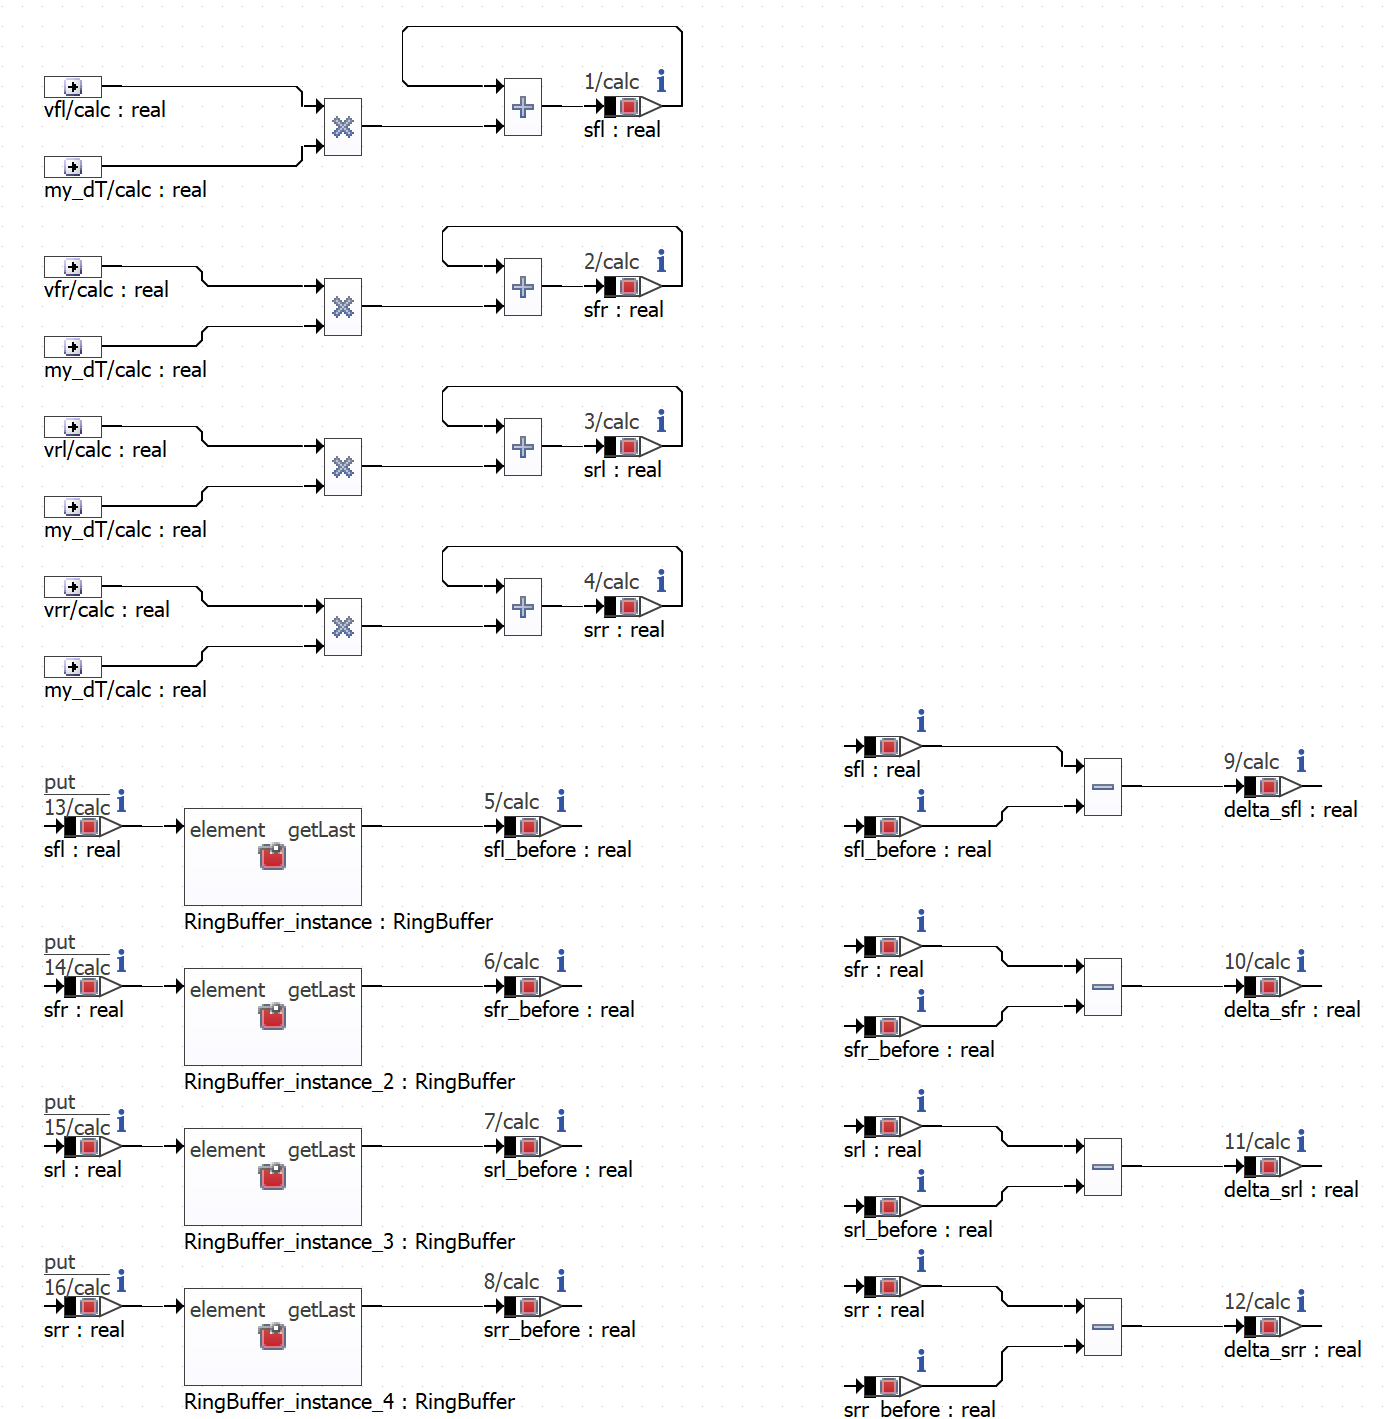
\includegraphics[width=1\linewidth]{../Graphiken/Model.png}
	\caption{Model}
	\label{fig:Model}
\end{figure}

Die \autoref{fig:TireMean} zeigt die Berechnung des Durchschnitts der vier Strecken.

\begin{figure}[h!]
	\centering
	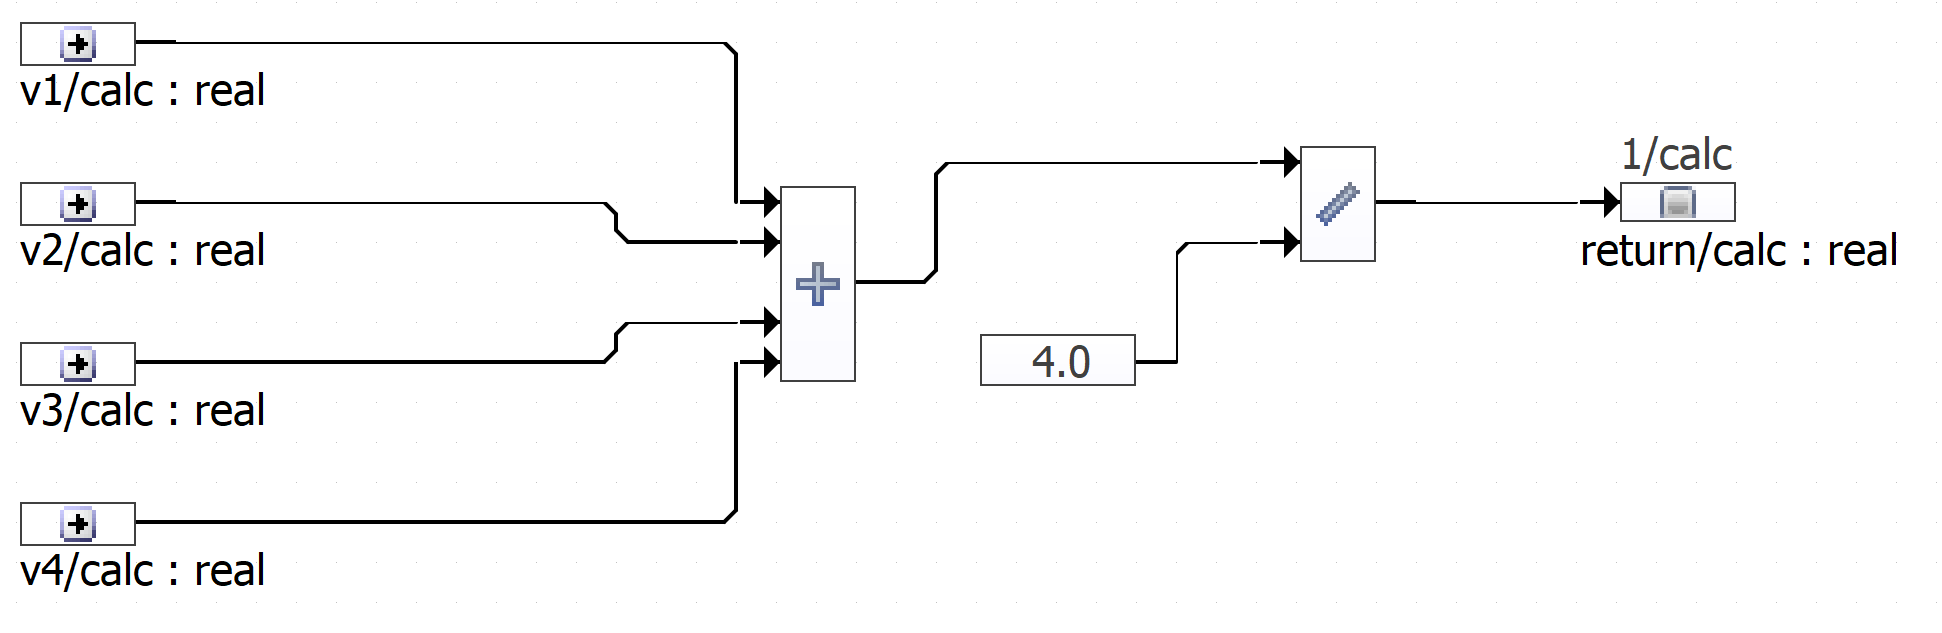
\includegraphics[width=1\linewidth]{../Graphiken/TireMean.png}
	\caption{Tire Mean}
	\label{fig:TireMean}
\end{figure}

\pagebreak
Die \autoref{fig:RandomGenerator} zeigt den \glqq Random Number Generator"' umgesetzt in ASCET.
Der anschließende Code zeigt, wie die Parameter a, m und c initialisiert wurden. Bei der Codegenerierung mit m = $2^{31}$ ist ein Fehler aufgetreten. Die Vermutung ist, dass dieser Wert zu groß ist. Deshalb wurde m auf $2^{10}$ gesetzt.\\
\begin{lstlisting}
class RandomGenerator {
	characteristic myint a = 89;
	characteristic myint m = 1024;
	characteristic myint c = 251;
	myint seed;
	myint x = 0;
	@generated("blockdiagram")
	public real calc(real in set_vel, real in noiselevel, integer in mySeed) {
		...
	}
}
\end{lstlisting}

\begin{figure}[h!]
	\centering
	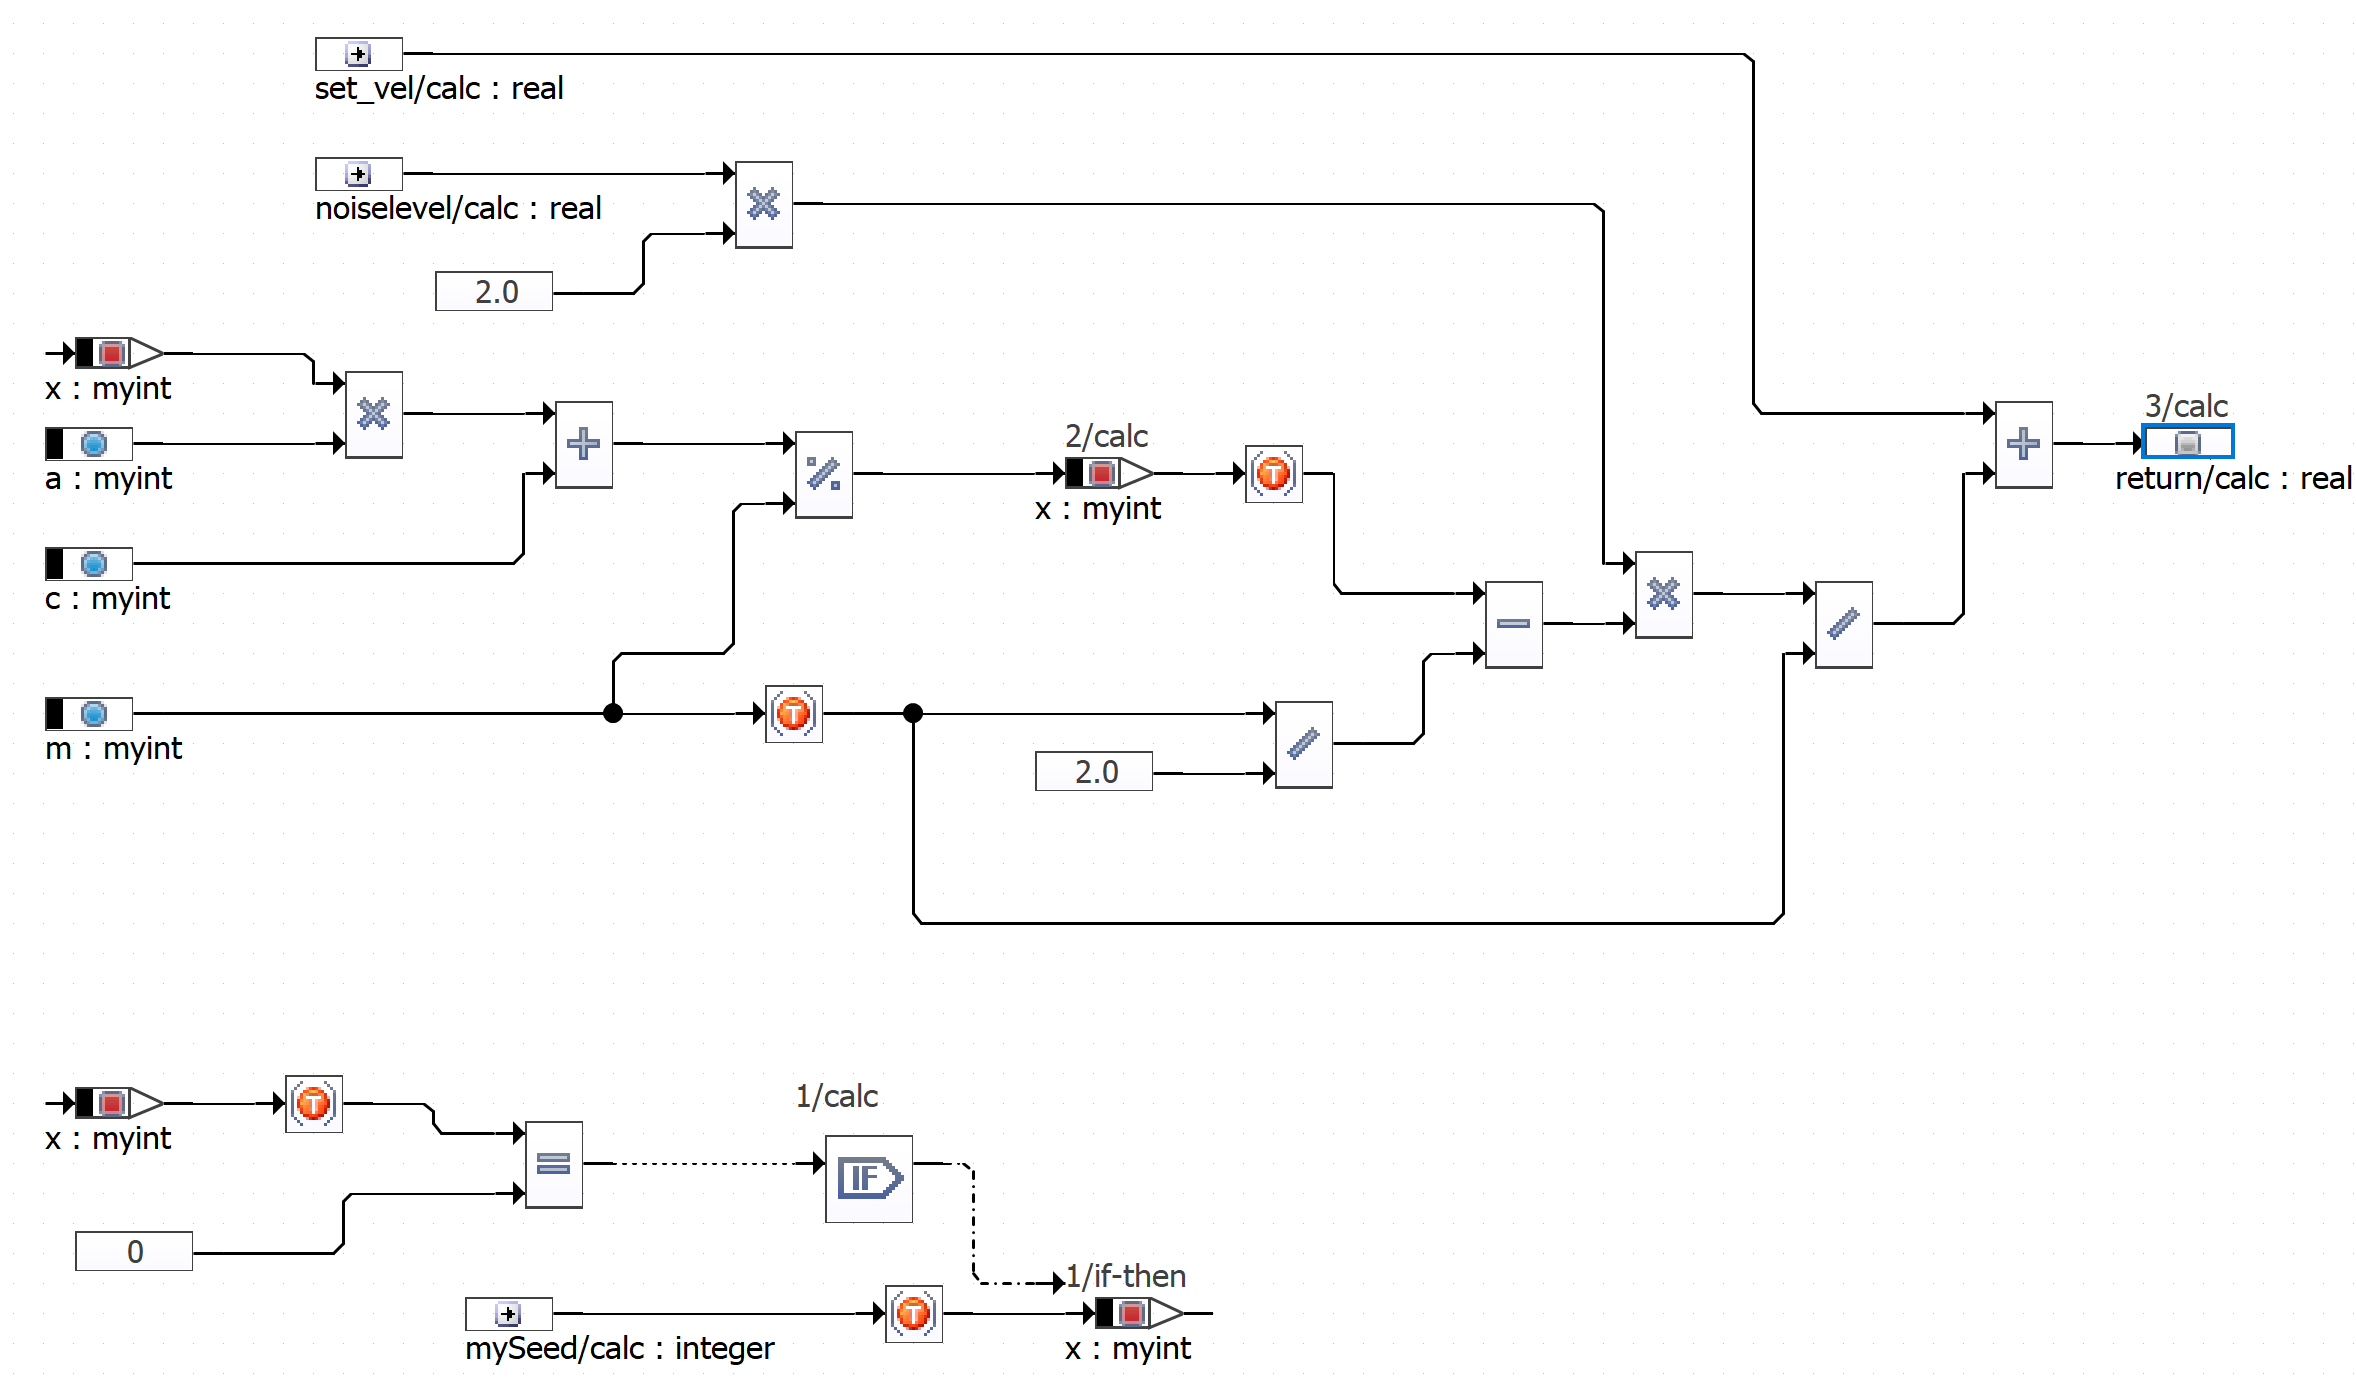
\includegraphics[width=1\linewidth]{../Graphiken/RandomGenerator.png}
	\caption{Random Number Generator}
	\label{fig:RandomGenerator}
\end{figure}